
\section{Calculations \& Graphs}

\vspace{-0.5cm}
\singlespacing

%------- Force --------%

%------- ACCELERATION BETWEEN TWO POINTS WITH INITIAL VELOCITY CLOSE TO ZERO--------%

\subsection{Period of a Spring with A Hanging Mass} 

{\centering
\begin{equation}
	\text{T} = 2\pi \sqrt{\frac{m}{k}}
	\label{eq:springMass}
\end{equation}
\begin{align*}
	\text{T} &: \text{period} \\
	m &: \text{mass of hanging weight and spring} \\
	k &: \text{spring constant}
\end{align*}}

\subsubsection{Sample Calculation \\ {\normalfont \small\textit{part 2, expected period for mass of 15 g}}}

{\centering
\begin{align*}
	\text{T} &= 2\pi \sqrt{\frac{m}{k}} \\ \\
					 &= 2\pi \sqrt{\frac{0.31\text{ kg}}{8.0051}} \\ \\
	\text{T}  &= \boxed{1.236\,\text{s}}
\end{align*}}

\subsection{Period of a Pendulum} 

{\centering
\begin{equation}
	\text{T} = 2\pi \sqrt{\frac{l}{g}}
	\label{eq:pendulum}
\end{equation}
\begin{align*}
	\text{T} &: \text{period} \\
	l &: \text{length of pendulum} \\
	g &: \text{acceleration due to gravity}
\end{align*}}

\vspace{-1.0cm}

\subsubsection{Sample Calculation \\ {\normalfont \small\textit{part 2, expected period for ideal pendulum}}}

{\centering
\begin{align*}
	\text{T} &= 2\pi \sqrt{\frac{l}{g}} \\
					 &= 2\pi \sqrt{\frac{1\text{ m}}{9.8\text{ m/s\textsuperscript{2}}}} \\
	\text{T}  &= \boxed{2\,\text{ s}}
\end{align*}}

%------- ACCELERATION BETWEEN TWO POINTS --------%

%------- AVERAGE VALUE --------%


\subsection{Fractional Discrepancy}
\vspace{0.5cm}
\begin{equation}
	\text{FD}	= \left| \frac{\text{measured - actual}}{\text{actual}} \right|\
	\label{eq:fdisc}
\end{equation}

\subsubsection{Sample Calculation \\ {\normalfont \small\textit{percent error between ideal period and measured period using values from part 3}}}

\begin{align*}
	\text{FD}	&= \left| \frac{\text{measured - actual}}{\text{actual}} \right|\ \\ \\
	\text{FD}	&= \left| \frac{\text{1.986\text{ s} - 2\text{ s}}}{\text{2\text{ s}}} \right|\ \\ \\
	\text{FD} &= \boxed{0.007} 
\end{align*}
%------- AVERAGE VALUE --------%

%------- STANDARD DEVIATION --------%
%\subsection{Standard Deviation Formula}
%
%\begin{align*}
%		\sigma &= \sqrt{\frac{\Sigma(x_i -\overline{a})^2}{N}} \\
%		 &= \sqrt{\frac{SS}{N}} \\ \\
%		\textbf{N} &:\, \text{Total number of values} \\
%		\overline{\textbf{a}} &:\, \text{Average value} \\
%		\textbf{x\textsubscript{i}} &:\, \text{Each value from the data set} \\
%		\textbf{SS} &:\, \text{Sum of squares} 
%\end{align*}
%
%\subsubsection{Sample Calculation \\ {\normalfont \small\textit{std of photogate times with hanging mass at 10 grams }}}
%
%\begin{align*}
%	\sigma &= \sqrt{\frac{(1.461-\overline{a})^2 + ... + (1.454-\overline{a})^2}{3}} \\
%				 &= \sqrt{\frac{2.886\,\text{x}\,10^{-5}}{3}} \\
%		 &= \boxed{0.0003\, \text{s}}
%\end{align*}
%------- STANDARD DEVIATION --------%

%------- RELATIVE ERROR --------%
\subsection{Percent Error}
\vspace{0.5cm}
\begin{equation}
	\text{PD}	= \left| \frac{\text{measured - actual}}{\text{actual}} \right|\: \text{x}\: 100\%
	\label{eq:perror}
\end{equation}

\subsubsection{Sample Calculation \\ {\normalfont \small\textit{percent error between ideal period and measured period using values from part 3}}}

\begin{align*}
	\text{PD}	&= \left| \frac{\text{measured - actual}}{\text{actual}} \right|\: \text{x}\: 100\% \\ \\
	\text{PD}	&= \left| \frac{\text{1.986\text{ s} - 2\text{ s}}}{\text{2\text{ s}}} \right|\: \text{x}\: 100\% \\ \\
	\text{PD} &= \boxed{0.7\%} 
\end{align*}
%------- RELATIVE ERROR --------%

%----TABLES-----%
\subsection{Tables}

\begin{table} [H]
\centering
\captionsetup{font=large}
\caption{Part 1 - Spring Constant Table}
\label{tab:p1tab}
\resizebox{\linewidth}{!}{%
\begin{tabular}{ccccccccc} 
\toprule
\textbf{Mass (kg)}    & 0.05  & 0.1   & 0.15  & 0.2   & 0.25  & 0.3   & 0.35  & 0.4    \\ 
\toprule
\textbf{Weight (N)}   & 0.49  & 0.98  & 1.47  & 1.96  & 2.45  & 2.94  & 3.43  & 3.92   \\
\textbf{Position (m)} & 0.555 & 0.615 & 0.675 & 0.735 & 0.795 & 0.855 & 0.915 & 0.989  \\ 
\toprule
\multicolumn{9}{c}{\textbf{\textbf{Mass of Spring (kg)}} 0.16}                         \\
\bottomrule
\end{tabular}
}
\end{table}

\begin{table}[H]
\centering
\captionsetup{font=large}
\caption{Part 2 - Periods of Different Hanging Masses}
\label{tab:p2tab}
\resizebox{\linewidth}{!}{%
\begin{tabular}{ccccc} 
\toprule
\textbf{Mass (kg)}              & 0.15   & 0.25   & 0.35   & 0.45    \\ 
\toprule
\textbf{Period (s)}             & 1.19   & 1.38   & 1.55   & 1.68    \\
\textbf{Measured T (s)}         & 1.19   & 1.38   & 1.55   & 1.68    \\
\textbf{Predicted T (s)}        & 1.236  & 1.421  & 1.585  & 1.734   \\ 
\toprule
\textbf{Fractional Discrepancy} & 0.0375 & 0.0295 & 0.0226 & 0.0313  \\
\bottomrule
\end{tabular}
}
\end{table}

\begin{table}[H]
\centering
\captionsetup{font=large}
\caption{Part 3 - Period of A Pendulum}
\label{tab:p3tab}
\resizebox{\linewidth}{!}{%
\begin{tabular}{cccc} 
\toprule
\textbf{Time for 5 Cycles (s)}                 & 9.93  & 9.89  & 9.93   \\ 
\toprule
\textbf{Measured T (s)}                        & 1.986 & 1.978 & 1.986  \\
\textbf{Ideal T (s)}                           & 2     & 2     & 2      \\
\textbf{Real T (s)}                            & 1.778 & 1.754 & 1.756  \\ 
\toprule
\textbf{~Error Between Measured \& Ideal (\%)} & 0.7   & 1.1   & 0.7    \\
\textbf{Error Between Measured \& Real (\%)~}  & 11.69 & 12.77 & 13.09  \\
\bottomrule
\end{tabular}
}
\end{table}
%----TABLES-----%

\begin{landscape}
\subsection{Graphs}
\vspace{-1cm}
\begin{figure}[H]
	\captionsetup{font=Large}
	\caption{Part 1: Spring Constant}
	\begin{center}
		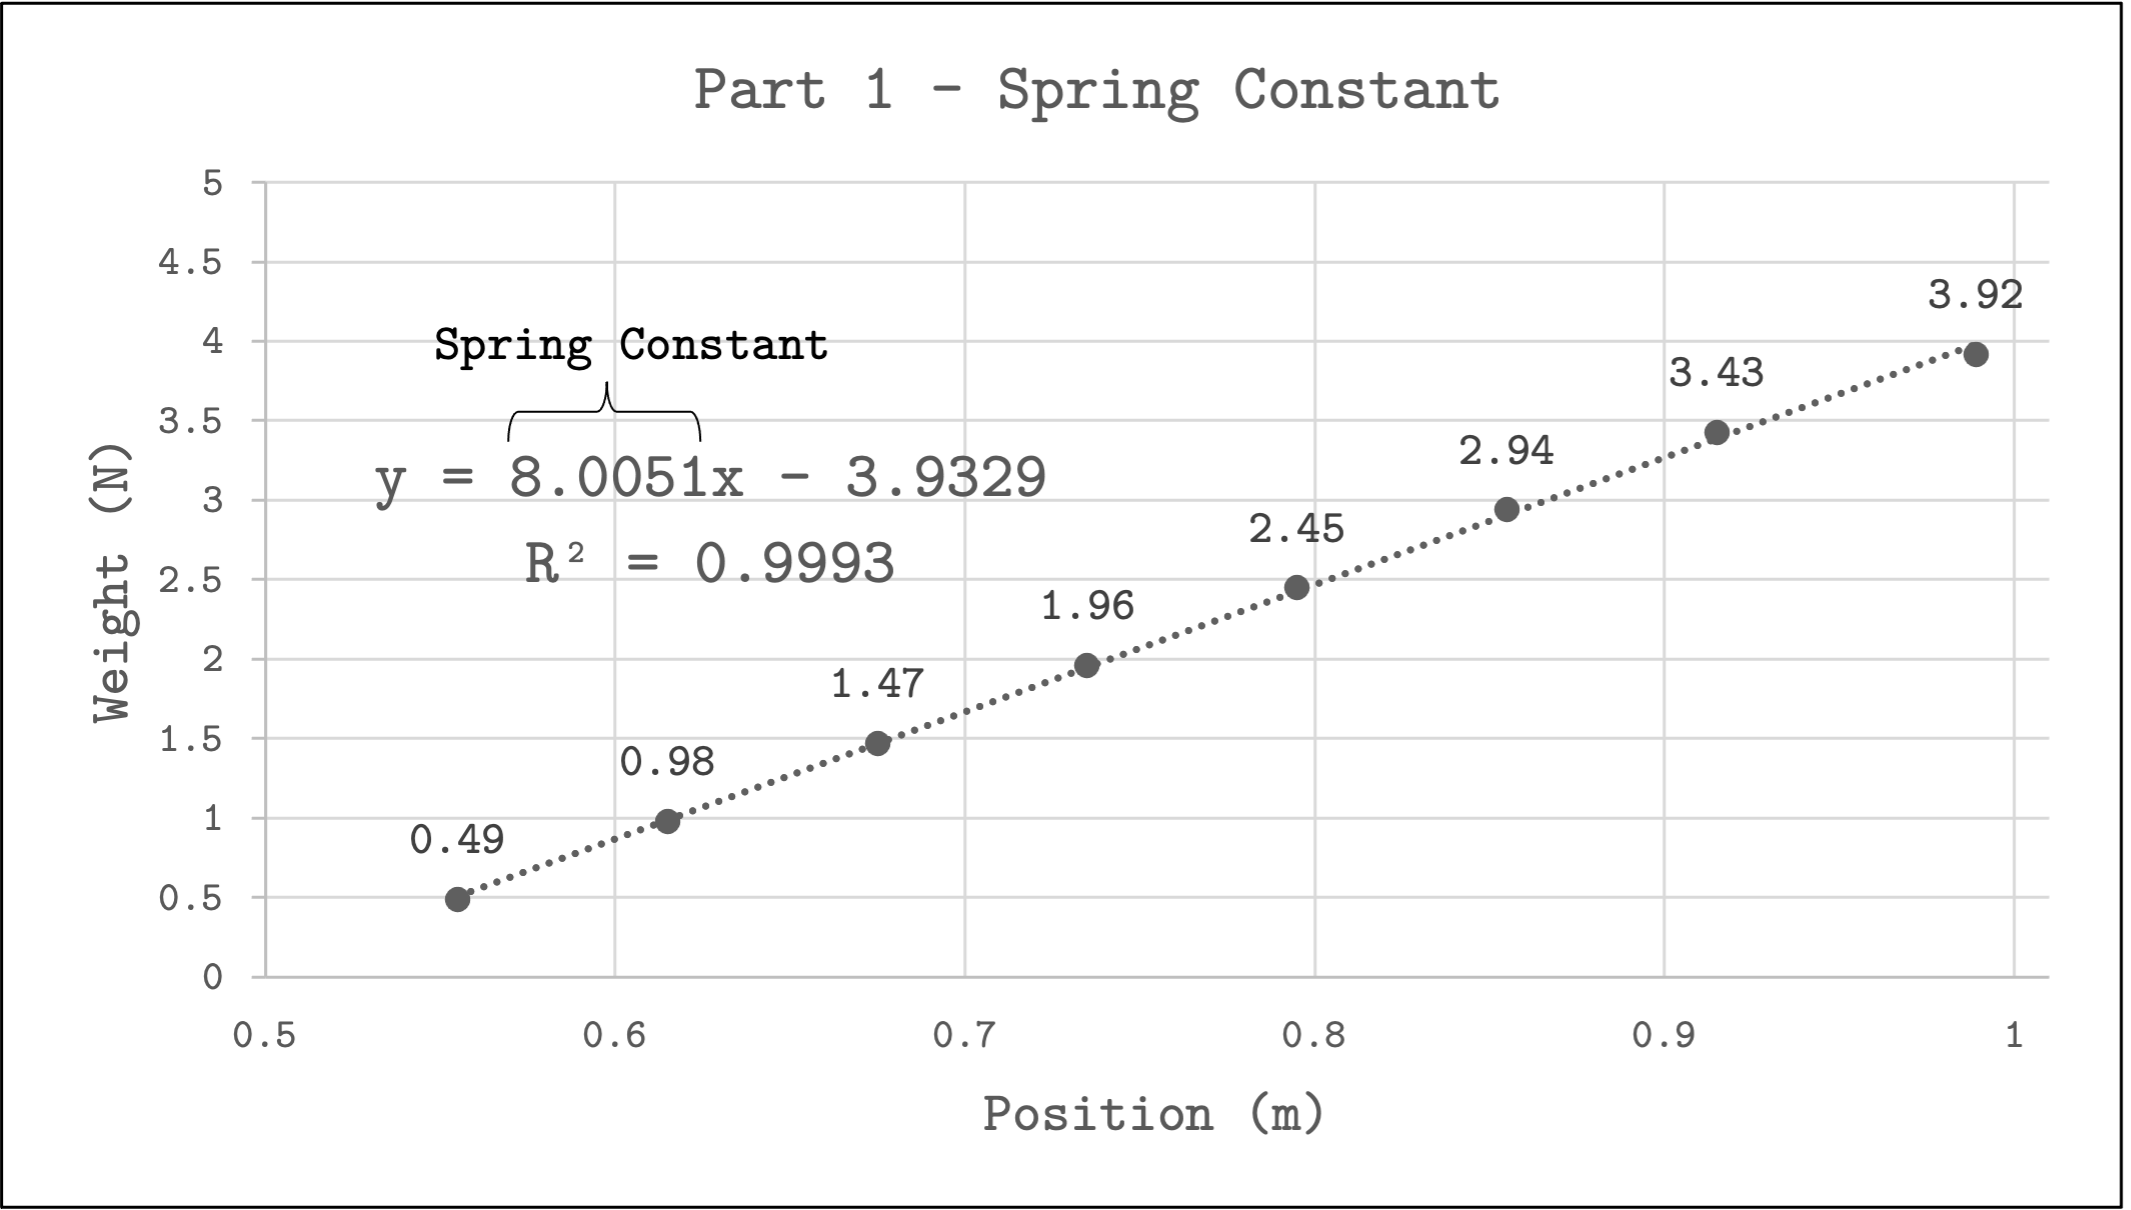
\includegraphics[width=0.90\columnwidth]{p1graph.png}
	\end{center}
	\label{fig:p1Graph}
\end{figure}

\end{landscape}

%----GRAPHS-----%

\newpage

